\documentclass{article}
\usepackage[utf8]{inputenc}
\usepackage{graphicx}
\usepackage{hyperref}
\usepackage{geometry}
\geometry{a4paper} % Set the page size to A4
\usepackage{listings} % Package for including code in the document

\title{Práctica 07: Funciones en SQL}
\author{Carlos I. Padilla Herrera}
\date{13 de mayo de 2024}

\lstset{frame=single, % Adds a frame around the code
        basicstyle=\small\ttfamily, % Use a small, true type font
        language=SQL, % SQL syntax highlighting
        showstringspaces=false} % Don't mark spaces in strings

\begin{document}

\begin{titlepage}
    \centering
    \vspace*{1cm}
    \Huge\textbf{Curso de base de datos entre semana G0224}
    
    \vspace{0.5cm}
    \LARGE Escuela de Código PILARES
    
    \vspace{1.5cm}
    \textbf{Carlos Ignacio Padilla Herrera}
    
    \vspace{2cm}
    \Large\textbf{Folio:} 794DR02
    
    \vspace{0.5cm}
    \Large\textbf{Proyecto final} Base de datos de proveedores.
    
    \vfill
    
    \Large\textbf{Fecha:} 13 de mayo de 2024.
    
    \vspace{0.8cm}
\end{titlepage}

\newpage

\section*{Diagrama entidad relación}


\begin{figure}[ht]
    \centering
    {
        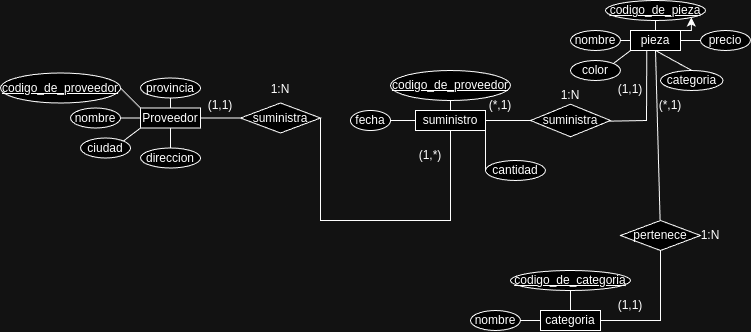
\includegraphics[width=\linewidth]{edc-proyecto-final.png} % Asegúrate de que el nombre del archivo y la extensión son correctos
    }
    \caption{Diagrama entidad relación del proyecto final}
\end{figure}

\newpage


\section*{Modelo entidad relación}


\begin{figure}[ht]
    \centering
    {
        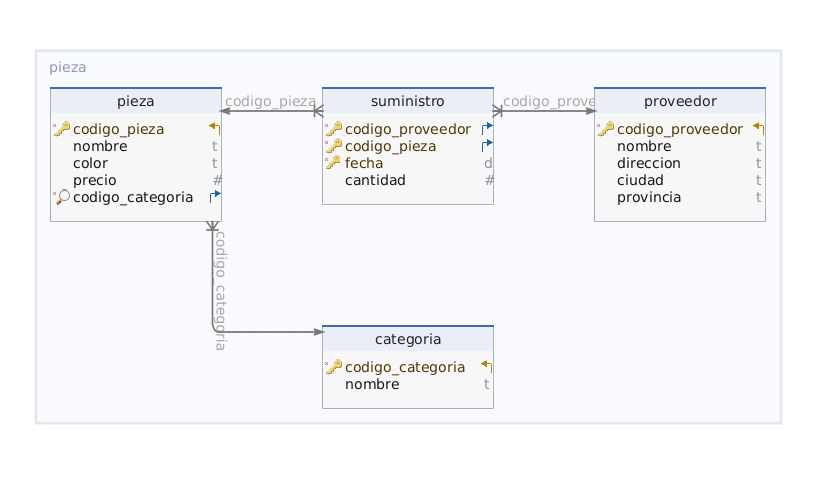
\includegraphics[width=\linewidth]{schema.png} % Asegúrate de que el nombre del archivo y la extensión son correctos
    }
    \caption{Esquema de la base de datos.}
\end{figure}

\newpage

\section*{Código SQL para la creación la base de datos y tablas}

\begin{lstlisting}
    create database if not exists proveedoresdb;
    use proveedoresdb;
    
    create table proveedor (
      codigo_proveedor varchar(255) not null,
      nombre varchar(255),
      direccion varchar(255),
      ciudad varchar(255),
      provincia varchar(255),
      primary key (codigo_proveedor)
    );
    
    create table categoria (
      codigo_categoria varchar(255) not null,
      nombre varchar(255),
      primary key (codigo_categoria)
    );
    
    create table pieza (
      codigo_pieza varchar(255) not null,
      nombre varchar(255),
      color varchar(255),
      precio decimal(10, 2),
      codigo_categoria varchar(255) not null,
      primary key (codigo_pieza),
      foreign key (codigo_categoria) references categoria(codigo_categoria)
    );
    
    create table suministro (
      codigo_proveedor varchar(255) not null,
      codigo_pieza varchar(255) not null,
      fecha date,
      cantidad int,
      primary key (codigo_proveedor, codigo_pieza, fecha),
      foreign key (codigo_proveedor) references proveedor(codigo_proveedor),
      foreign key (codigo_pieza) references pieza(codigo_pieza)
    );
    
\end{lstlisting}

\newpage % Inicia una nueva página



\newpage % Inicia una nueva página

\section*{Lista  de las piezas que cada proveedor suministra}

\begin{figure}[ht]
    \centering
    {
        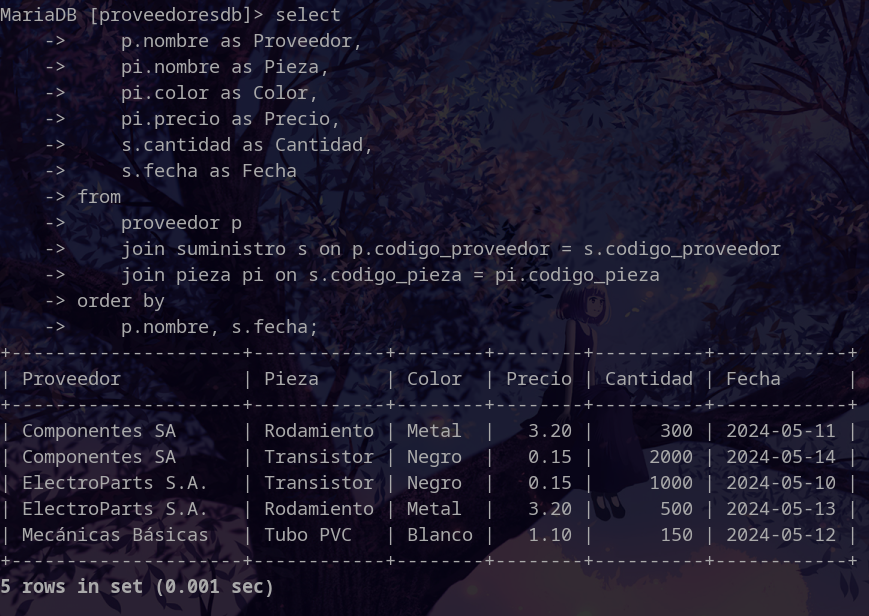
\includegraphics[width=\linewidth]{01screenshot.png} % Asegúrate de que el nombre del archivo y la extensión son correctos
    }
    \caption{Subconsulta para saber que piezas suministra cada proveedor.}
\end{figure}


\end{document}
